\documentclass[a4paper,12pt]{report}

\usepackage[utf8]{vietnam}

\usepackage{amsmath}
\usepackage{geometry}
\geometry{
    top=2.5cm,
    bottom=2.5cm,
    left=3cm,
    right=2cm,
}

\usepackage{graphicx}
\usepackage{xcolor}
\usepackage{hyperref}
\hypersetup{
    colorlinks=true,
    linkcolor=blue,
    urlcolor=blue,
    citecolor=blue,
}

\usepackage{tikz}
\usetikzlibrary{shapes.geometric, arrows, positioning, fit, backgrounds, calc}

\usepackage{booktabs}
\usepackage{array}
\usepackage{longtable}
\usepackage{multirow}
\usepackage{verbatim}

\usepackage{listings}
\lstset{
    basicstyle=\ttfamily\small,
    breaklines=true,
    tabsize=4,
    numbers=left,
    numberstyle=\tiny,
    frame=single,
    language=C++,
    keywordstyle=\color{blue}\bfseries,
    commentstyle=\color{green!60!black},
    stringstyle=\color{red},
}

\usepackage{titlesec}
\titleformat{\chapter}[display]
  {\bfseries\Large}
  {\chaptername\ \thechapter}
  {20pt}{\Huge}

\usepackage{fancyhdr}
\setlength{\headheight}{18pt}
\pagestyle{fancy}
\fancyhf{}
\fancyhead[L]{\leftmark}
\fancyhead[R]{\thepage}
\fancyfoot[C]{}
\renewcommand{\headrulewidth}{0.4pt}

\usepackage{tocloft}
\renewcommand{\cfttoctitlefont}{\huge\bfseries}

\newcommand{\code}[1]{\texttt{\hyphenchar\font=45\relax#1}}

\begin{document}

\begin{titlepage}
\begin{center}

\vspace*{1cm}

{\Large TRƯỜNG ĐẠI HỌC ...}\\[0.3cm]
{\large KHOA ...}\\[0.3cm]
{\large BỘ MÔN ...}\\[1.5cm]

\rule{\textwidth}{1pt}\\[0.5cm]
{\Huge \bfseries BÁO CÁO ĐỒ ÁN}\\[0.3cm]
{\Large Mô phỏng các thuật toán điều phối tiến trình}\\[0.2cm]
{\large \textit{Process Scheduling Algorithm Simulator}}\\[0.3cm]
\rule{\textwidth}{1pt}\\[1.5cm]

\vfill

\begin{tabular}{l l}
Học viên thực hiện: & \textbf{Nguyễn Văn A} \\
Mã số: & 12345678 \\
Lớp: & ... \\
Giảng viên hướng dẫn: & \textbf{TS. Nguyễn Văn B} \\
\end{tabular}

\vfill

{\large Thành phố Hồ Chí Minh, 2025}

\end{center}
\end{titlepage}


\pagenumbering{roman}
\tableofcontents
\newpage

\listoffigures
\newpage

\listoftables
\newpage

\pagenumbering{arabic}

\chapter{Tổng quan đề tài}

\section{Giới thiệu bài toán điều phối tiến trình}

Trong hệ điều hành hiện đại, CPU là tài nguyên quan trọng nhất và cần được quản lý một cách hiệu quả. Điều phối tiến trình (process scheduling) là cơ chế mà hệ điều hành sử dụng để quyết định tiến trình nào sẽ được cấp CPU tại một thời điểm nhất định. Mục tiêu của điều phối tiến trình là tối ưu hóa hiệu suất hệ thống thông qua các chỉ số như thời gian đáp ứng (response time), thời gian chờ (waiting time), thời gian quay vòng (turnaround time) và mức độ sử dụng tài nguyên (utilization).

Có nhiều thuật toán điều phối khác nhau, mỗi thuật toán phù hợp với một loại hệ thống và mục tiêu thiết kế riêng:
\begin{itemize}
    \item \textbf{FCFS (First-Come, First-Served):} Thuật toán đơn giản nhất, tiến trình đến trước được phục vụ trước.
    \item \textbf{RR (Round Robin):} Mỗi tiến trình được cấp CPU trong một khoảng thời gian cố định (quantum), đảm bảo tính công bằng.
    \item \textbf{SJF (Shortest Job First):} Tiến trình có tổng thời gian CPU ngắn nhất được ưu tiên thực thi trước.
    \item \textbf{SRTN (Shortest Remaining Time Next):} Biến thể preemptive của SJF, tiến trình có thời gian CPU còn lại ngắn nhất được ưu tiên.
\end{itemize}

Ngoài CPU, các tài nguyên khác như thiết bị nhập/xuất, bộ nhớ dùng chung cũng cần được điều phối. Đồ án này mô phỏng một hệ thống có một CPU và một tài nguyên dùng chung R (Resource), nơi tài nguyên R được điều phối theo cơ chế FCFS.

\section{Mục tiêu đồ án}

Đồ án nhằm các mục tiêu sau:

\begin{enumerate}
    \item \textbf{Xây dựng chương trình mô phỏng} hoạt động điều phối tiến trình với 4 thuật toán: FCFS, Round Robin, SJF và SRTN.
    \item \textbf{Hỗ trợ tài nguyên dùng chung R:} Mỗi tiến trình có thể yêu cầu CPU và tài nguyên R nhiều lần, xen kẽ theo chu kỳ CPU-R.
    \item \textbf{Xuất biểu đồ Gantt:} Hiển thị trực quan thứ tự thực thi trên CPU và tài nguyên R.
    \item \textbf{Phân tích hiệu năng:} Tính toán các chỉ số response time, waiting time, turnaround time và utilization cho mỗi thuật toán.
    \item \textbf{Giao diện trực quan:} Cung cấp chế độ TUI (Terminal User Interface) để quan sát quá trình mô phỏng theo thời gian thực.
\end{enumerate}

\section{Phạm vi và giới hạn}

\subsection{Phạm vi}
\begin{itemize}
    \item Hệ thống mô phỏng hoạt động ở mức độ rời rạc (discrete-time simulation), mỗi đơn vị thời gian là một tick.
    \item Hỗ trợ đầy đủ 4 thuật toán điều phối CPU.
    \item Hỗ trợ 1 tài nguyên R với cơ chế FCFS.
    \item Đầu vào là file văn bản với cấu trúc đơn giản, đầu ra là biểu đồ Gantt.
\end{itemize}

\subsection{Giới hạn}
\begin{itemize}
    \item Chưa hỗ trợ các thuật toán nâng cao như MLFQ (Multi-Level Feedback Queue) hay Priority Scheduling.
    \item Chỉ mô phỏng một tài nguyên R duy nhất.
    \item Chưa tính đến overhead của context-switch.
    \item Chưa có cơ chế phát hiện starvation cho các thuật toán SJF và SRTN.
\end{itemize}

\section{Cấu trúc báo cáo}

Báo cáo được tổ chức thành 6 chương:
\begin{itemize}
    \item \textbf{Chương 1 - Tổng quan đề tài:} Giới thiệu bài toán, mục tiêu và phạm vi.
    \item \textbf{Chương 2 - Cơ sở lý thuyết:} Trình bày các khái niệm nền tảng về điều phối tiến trình và các thuật toán.
    \item \textbf{Chương 3 - Phân tích và thiết kế:} Mô tả kiến trúc, các lớp và mối quan hệ giữa chúng.
    \item \textbf{Chương 4 - Giải thích cài đặt:} Đi sâu vào chi tiết triển khai các thành phần chính.
    \item \textbf{Chương 5 - Kết quả thực nghiệm:} Trình bày kết quả chạy test với các bộ dữ liệu mẫu.
    \item \textbf{Chương 6 - Kết luận:} Đánh giá kết quả đạt được và hướng phát triển.
\end{itemize}

\chapter{Cơ sở lý thuyết}

\section{Khái niệm tiến trình}

Tiến trình (process) là một chương trình đang trong quá trình thực thi. Mỗi tiến trình trong hệ điều hành được quản lý thông qua một khối dữ liệu gọi là Process Control Block (PCB), chứa các thông tin như:
\begin{itemize}
    \item Process ID (PID): định danh duy nhất của tiến trình.
    \item Trạng thái (state): new, ready, running, waiting, terminated.
    \item Program Counter: địa chỉ lệnh tiếp theo sẽ thực thi.
    \item CPU registers: các thanh ghi cần lưu lại khi chuyển đổi ngữ cảnh.
    \item Thông tin điều phối: độ ưu tiên, thời gian chờ, thời gian CPU đã dùng.
\end{itemize}

Trong mô hình điều phối, mỗi tiến trình luân phiên thực hiện các chu kỳ CPU burst và I/O burst (hoặc Resource burst). Một CPU burst là khoảng thời gian tiến trình sử dụng CPU để tính toán, trong khi Resource burst là khoảng thời gian tiến trình truy cập tài nguyên (như thiết bị nhập/xuất, bộ nhớ dùng chung).

\begin{figure}[h]
\centering
\begin{tikzpicture}[node distance=0.5cm]
\tikzstyle{box}=[rectangle, draw, minimum width=1.8cm, minimum height=0.8cm, rounded corners]
\tikzstyle{cpu}=[box, fill=blue!20]
\tikzstyle{res}=[box, fill=green!20]

\node[cpu] (c1) {CPU 5};
\node[res, right=0.3cm of c1] (r1) {R 2};
\node[cpu, right=0.3cm of r1] (c2) {CPU 3};
\node[res, right=0.3cm of c2] (r2) {R 1};
\node[cpu, right=0.3cm of r2] (c3) {CPU 4};

\draw[->, thick] (c1) -- (r1);
\draw[->, thick] (r1) -- (c2);
\draw[->, thick] (c2) -- (r2);
\draw[->, thick] (r2) -- (c3);

\node[below=0.3cm of c1] {\small tick 0--5};
\node[below=0.3cm of r1] {\small tick 5--7};
\node[below=0.3cm of c2] {\small tick 7--10};
\node[below=0.3cm of r2] {\small tick 10--11};
\node[below=0.3cm of c3] {\small tick 11--15};
\end{tikzpicture}
\caption{Ví dụ chu kỳ CPU-R của một tiến trình}
\label{fig:cpu-r-cycle}
\end{figure}

\section{Các thuật toán điều phối CPU}

\subsection{FCFS (First-Come, First-Served)}

FCFS là thuật toán điều phối đơn giản nhất. Tiến trình nào đến trước sẽ được phục vụ trước. Thuật toán này hoạt động theo cơ chế non-preemptive: một khi tiến trình đã được cấp CPU, nó sẽ giữ CPU cho đến khi kết thúc CPU burst hiện tại hoặc tự nguyện nhả CPU để chuyển sang tài nguyên R.

\begin{quote}
\textbf{FCFS Scheduling}\\
Input: Ready queue $Q$\\
Output: Index of selected process\\
\begin{verbatim}
if Q is not empty:
    return 0   // Pick first (oldest) process
return -1      // No process to run
\end{verbatim}
\end{quote}

\textbf{Ưu điểm:} Đơn giản, dễ cài đặt.
\textbf{Nhược điểm:} Hiệu ứng convoy -- tiến trình CPU-bound dài làm chậm các tiến trình I/O-bound ngắn phía sau.

\subsection{Round Robin (RR)}

Round Robin là thuật toán preemptive, mỗi tiến trình được cấp CPU trong một khoảng thời gian cố định gọi là quantum (thường 10--100ms). Nếu tiến trình không hoàn thành CPU burst trong quantum đó, nó bị preempt và đưa trở lại cuối hàng đợi ready.

\begin{quote}
\textbf{Round Robin Scheduling (quantum $q$)}\\
Input: Ready queue $Q$, current process $P$, quantum counter $c$\\
Output: Next process for CPU\\
\begin{verbatim}
if P is null and Q is not empty:
    return 0              // Pick first in queue
if P is running and c >= q:
    PREEMPT(P)             // Move P back to Q
if P is null and Q not empty:
    return 0              // Pick next from queue
\end{verbatim}
\end{quote}

\textbf{Ưu điểm:} Công bằng, không bị starvation, phù hợp với hệ thống time-sharing.
\textbf{Nhược điểm:} Hiệu suất phụ thuộc nhiều vào quantum -- quantum quá nhỏ gây nhiều context-switch, quantum quá lớn làm RR trở thành FCFS.

\subsection{SJF (Shortest Job First -- Non-Preemptive)}

SJF chọn tiến trình có tổng thời gian CPU burst ngắn nhất trong hàng đợi ready để thực thi. Đây là thuật toán non-preemptive: một khi tiến trình được chọn, nó chạy cho đến khi kết thúc CPU burst hoặc tự nguyện nhả CPU.

\begin{quote}
\textbf{SJF Scheduling (Non-Preemptive)}\\
Input: Ready queue $Q$\\
Output: Index of process with shortest remaining CPU\\
\begin{verbatim}
best_idx = 0
best_time = Q[0].getRemainingCPUTotal()
for i = 1 to |Q|-1:
    t = Q[i].getRemainingCPUTotal()
    if t < best_time:
        best_idx = i
        best_time = t
return best_idx
\end{verbatim}
\end{quote}

\textbf{Ưu điểm:} Tối ưu thời gian chờ trung bình (minimizes average waiting time).
\textbf{Nhược điểm:} Có thể gây starvation cho tiến trình có burst dài; khó dự đoán độ dài CPU burst trong thực tế.

\subsection{SRTN (Shortest Remaining Time Next -- Preemptive)}

SRTN là phiên bản preemptive của SJF. Tại mỗi thời điểm, nếu có một tiến trình trong hàng đợi ready có tổng thời gian CPU còn lại nhỏ hơn tiến trình đang chạy, tiến trình đang chạy sẽ bị preempt.

\begin{quote}
\textbf{SRTN Scheduling (Preemptive)}\\
Input: Ready queue $Q$, current process $P$\\
Output: Next process for CPU\\
\begin{verbatim}
if P is null and Q is not empty:
    return findShortest(Q)
if P is running and Q is not empty:
    shortest = findShortest(Q)
    if Q[shortest].getRemainingCPUTotal()
         < P.getRemainingCPUTotal():
        PREEMPT(P)
        return shortest
\end{verbatim}
\end{quote}

\textbf{Ưu điểm:} Tối ưu thời gian chờ trung bình hơn SJF nhờ tính preemptive.
\textbf{Nhược điểm:} Càng dễ gây starvation hơn SJF; chi phí tính toán và preemption cao hơn.

\section{Bài toán tài nguyên dùng chung}

Trong hệ thống thực, tiến trình không chỉ sử dụng CPU mà còn cần truy cập các tài nguyên khác như thiết bị nhập/xuất, bộ nhớ dùng chung, file, v.v. Đồ án này mô hình hóa một tài nguyên dùng chung R với cơ chế điều phối FCFS.

Khi một tiến trình hoàn thành CPU burst và burst tiếp theo là Resource R, nó được đưa vào hàng đợi resource. Resource R chỉ phục vụ một tiến trình tại một thời điểm. Khi tiến trình hoàn thành Resource burst, nó quay trở lại hàng đợi ready để tiếp tục cạnh tranh CPU.

Điều đặc biệt là CPU và Resource R hoạt động \textbf{độc lập}: một tiến trình có thể sử dụng Resource R trong khi tiến trình khác đang sử dụng CPU. Điều này phản ánh đúng kiến trúc của hệ thống thực nơi CPU và thiết bị I/O có thể hoạt động song song.

\section{Các chỉ số đánh giá hiệu năng}

\subsection{Các chỉ số trên từng tiến trình}

\begin{itemize}
    \item \textbf{Response Time ($RT_i$):} Thời gian từ khi tiến trình vào ready queue lần đầu đến khi được cấp CPU lần đầu tiên.
    \begin{equation}
        RT_i = \text{first\_response\_time}_i - \text{arrival\_time}_i
    \end{equation}
    
    \item \textbf{Waiting Time ($WT_i$):} Tổng thời gian tiến trình ở trong ready queue (chờ CPU).
    \begin{equation}
        WT_i = \sum \text{(thời gian chờ trong ready queue)}
    \end{equation}
    
    \item \textbf{Turnaround Time ($TAT_i$):} Thời gian từ khi tiến trình đến hệ thống đến khi hoàn thành.
    \begin{equation}
        TAT_i = \text{completion\_time}_i - \text{arrival\_time}_i
    \end{equation}
    
    \item \textbf{Mối quan hệ:} $TAT_i = WT_i + \text{(tổng CPU burst)} + \text{(tổng Resource burst)}$
\end{itemize}

\subsection{Các chỉ số hệ thống}

\begin{itemize}
    \item \textbf{CPU Utilization:} Phần trăm thời gian CPU hoạt động (không idle).
    \begin{equation}
        \text{CPU\_Util} = \left(1 - \frac{\text{total\_cpu\_idle\_time}}{\text{total\_simulation\_time}}\right) \times 100\%
    \end{equation}
    
    \item \textbf{Resource Utilization:} Phần trăm thời gian Resource R hoạt động.
    \begin{equation}
        \text{R\_Util} = \left(1 - \frac{\text{total\_res\_idle\_time}}{\text{total\_simulation\_time}}\right) \times 100\%
    \end{equation}
    
    \item \textbf{Trung bình hệ thống:}
    \begin{align}
        \overline{RT} &= \frac{1}{N} \sum_{i=1}^{N} RT_i \\
        \overline{WT} &= \frac{1}{N} \sum_{i=1}^{N} WT_i \\
        \overline{TAT} &= \frac{1}{N} \sum_{i=1}^{N} TAT_i
    \end{align}
\end{itemize}

\chapter{Phân tích và thiết kế}

\section{Yêu cầu chức năng}

Chương trình mô phỏng điều phối tiến trình đáp ứng các yêu cầu chức năng sau:

\begin{enumerate}
    \item \textbf{Đọc dữ liệu đầu vào:} Đọc file văn bản chứa thông tin các tiến trình (thời gian đến, chuỗi CPU burst và Resource burst).
    \item \textbf{Lựa chọn thuật toán:} Hỗ trợ 4 thuật toán FCFS, RR, SJF, SRTN thông qua tham số dòng lệnh hoặc menu tương tác.
    \item \textbf{Mô phỏng theo tick:} Chạy mô phỏng từng đơn vị thời gian, cập nhật trạng thái các tiến trình, CPU và tài nguyên R.
    \item \textbf{Xuất biểu đồ Gantt:} Ghi biểu đồ Gantt của CPU và tài nguyên R ra file đầu ra.
    \item \textbf{Phân tích hiệu năng:} Tính toán và hiển thị các chỉ số response time, waiting time, turnaround time và utilization.
    \item \textbf{Chế độ TUI:} Hiển thị trực quan quá trình mô phỏng theo thời gian thực (tùy chọn).
\end{enumerate}

\section{Kiến trúc tổng thể}

Chương trình được thiết kế theo mô hình hướng đối tượng với sự phân tách trách nhiệm rõ ràng giữa các lớp. Kiến trúc tổng thể tuân theo mẫu thiết kế Strategy cho phép dễ dàng thêm mới các thuật toán điều phối.

\begin{figure}[h]
\centering
\begin{tikzpicture}[node distance=1.2cm, scale=0.6, transform shape]
\tikzstyle{io}=[rectangle, draw, fill=orange!20, minimum width=2.2cm, minimum height=0.8cm, rounded corners, align=center, font=\small]
\tikzstyle{proc}=[rectangle, draw, fill=blue!20, minimum width=2.2cm, minimum height=0.8cm, rounded corners, align=center, font=\small]
\tikzstyle{data}=[rectangle, draw, fill=green!20, minimum width=2.2cm, minimum height=0.8cm, rounded corners, align=center, font=\small]
\tikzstyle{arrow}=[->, thick]

\node[io] (input) {Input File\\ (.txt)};
\node[proc, right=1.2cm of input] (parser) {Parser};
\node[data, right=1.2cm of parser] (processes) {vector<Process>};
\node[proc, right=1.2cm of processes] (scheduler) {Scheduler};
\node[proc, below=0.8cm of scheduler] (algo) {Algorithm\\ (Strategy)};
\node[data, right=1.2cm of scheduler] (gantt) {Gantt Data};
\node[proc, right=1.2cm of gantt] (output) {Parser\\ writeOutput};
\node[io, right=1.2cm of output] (outfile) {Output File\\ (Gantt)};
\node[proc, below=0.8cm of gantt] (analytics) {Analytics};
\node[proc, below=0.8cm of scheduler] (visualizer) {Visualizer\\ (TUI)};

\draw[arrow] (input) -- (parser);
\draw[arrow] (parser) -- (processes);
\draw[arrow] (processes) -- (scheduler);
\draw[arrow] (scheduler) -- (algo);
\draw[arrow] (scheduler) -- (gantt);
\draw[arrow] (gantt) -- (output);
\draw[arrow] (output) -- (outfile);
\draw[arrow] (gantt) -- (analytics);
\draw[arrow] (scheduler) -- (visualizer);

\end{tikzpicture}
\caption{Kiến trúc tổng thể của chương trình}
\label{fig:architecture}
\end{figure}

\section{Thiết kế chi tiết các lớp}

\subsection{Lớp Process và TaskBurst}

Lớp \code{Process} biểu diễn một tiến trình trong hệ thống. Mỗi tiến trình có một danh sách các \code{TaskBurst}, mỗi burst có thể là CPU hoặc RESOURCE.

\begin{itemize}
    \item \textbf{Thuộc tính chính:} PID, arrival\_time, danh sách burst, current\_burst\_index, thời gian đáp ứng, thời gian hoàn thành, thời gian chờ.
    \item \textbf{Phương thức chính:} \code{advanceBurst()} (chuyển burst tiếp theo), \linebreak[4]\code{getRemainingCPUTotal()} (tính tổng CPU còn lại), \code{markCompletion()}, \code{markFirstResponse()}, \code{addWaitingTime()}.
\end{itemize}

\subsection{Lớp ISchedulingAlgorithm (Interface)}

Đây là interface định nghĩa phương thức \code{pickNext()} -- chiến lược chọn tiến trình tiếp theo từ hàng đợi ready. Bốn lớp con cài đặt cụ thể:

\begin{itemize}
    \item \textbf{FCFSScheduler:} Luôn chọn tiến trình ở đầu hàng đợi (index 0).
    \item \textbf{RoundRobinScheduler:} Luôn chọn index 0, preemption do Scheduler xử lý.
    \item \textbf{SJFScheduler:} Duyệt hàng đợi, chọn tiến trình có \code{getRemainingCPUTotal()} nhỏ nhất.
    \item \textbf{SRTNScheduler:} Cùng logic SJF, nhưng Scheduler gọi \code{checkSRTNPreemption()} để preempt.
\end{itemize}

\subsection{Lớp Scheduler}

\code{Scheduler} là lớp trung tâm điều phối toàn bộ quá trình mô phỏng. Nó sở hữu danh sách tiến trình, hàng đợi ready, CPU state, tài nguyên R và con trỏ tới thuật toán điều phối.

\subsection{Lớp Resource}

\code{Resource} mô hình hóa tài nguyên dùng chung R với cơ chế FCFS. Nó duy trì hàng đợi resource, tiến trình đang sử dụng, lịch sử Gantt và thời gian idle.

\subsection{Lớp Parser}

\code{Parser} là lớp tiện ích tĩnh với hai phương thức:
\begin{itemize}
    \item \code{parseInput()}: Đọc file đầu vào, phân tích cú pháp, tạo danh sách \code{Process}.
    \item \code{writeOutput()}: Ghi biểu đồ Gantt CPU và Resource ra file đầu ra.
\end{itemize}

\subsection{Lớp Visualizer}

\code{Visualizer} cung cấp giao diện TUI real-time. Mỗi tick, nó nhận \code{SystemSnapshot} (trạng thái hệ thống tại tick đó) và render lên terminal với mã màu ANSI.

\subsection{Lớp Analytics}

\code{Analytics} nhận kết quả mô phỏng, tính toán các chỉ số hiệu năng và in báo cáo dạng bảng.

\section{Class Diagram}

\begin{figure}[h]
\centering
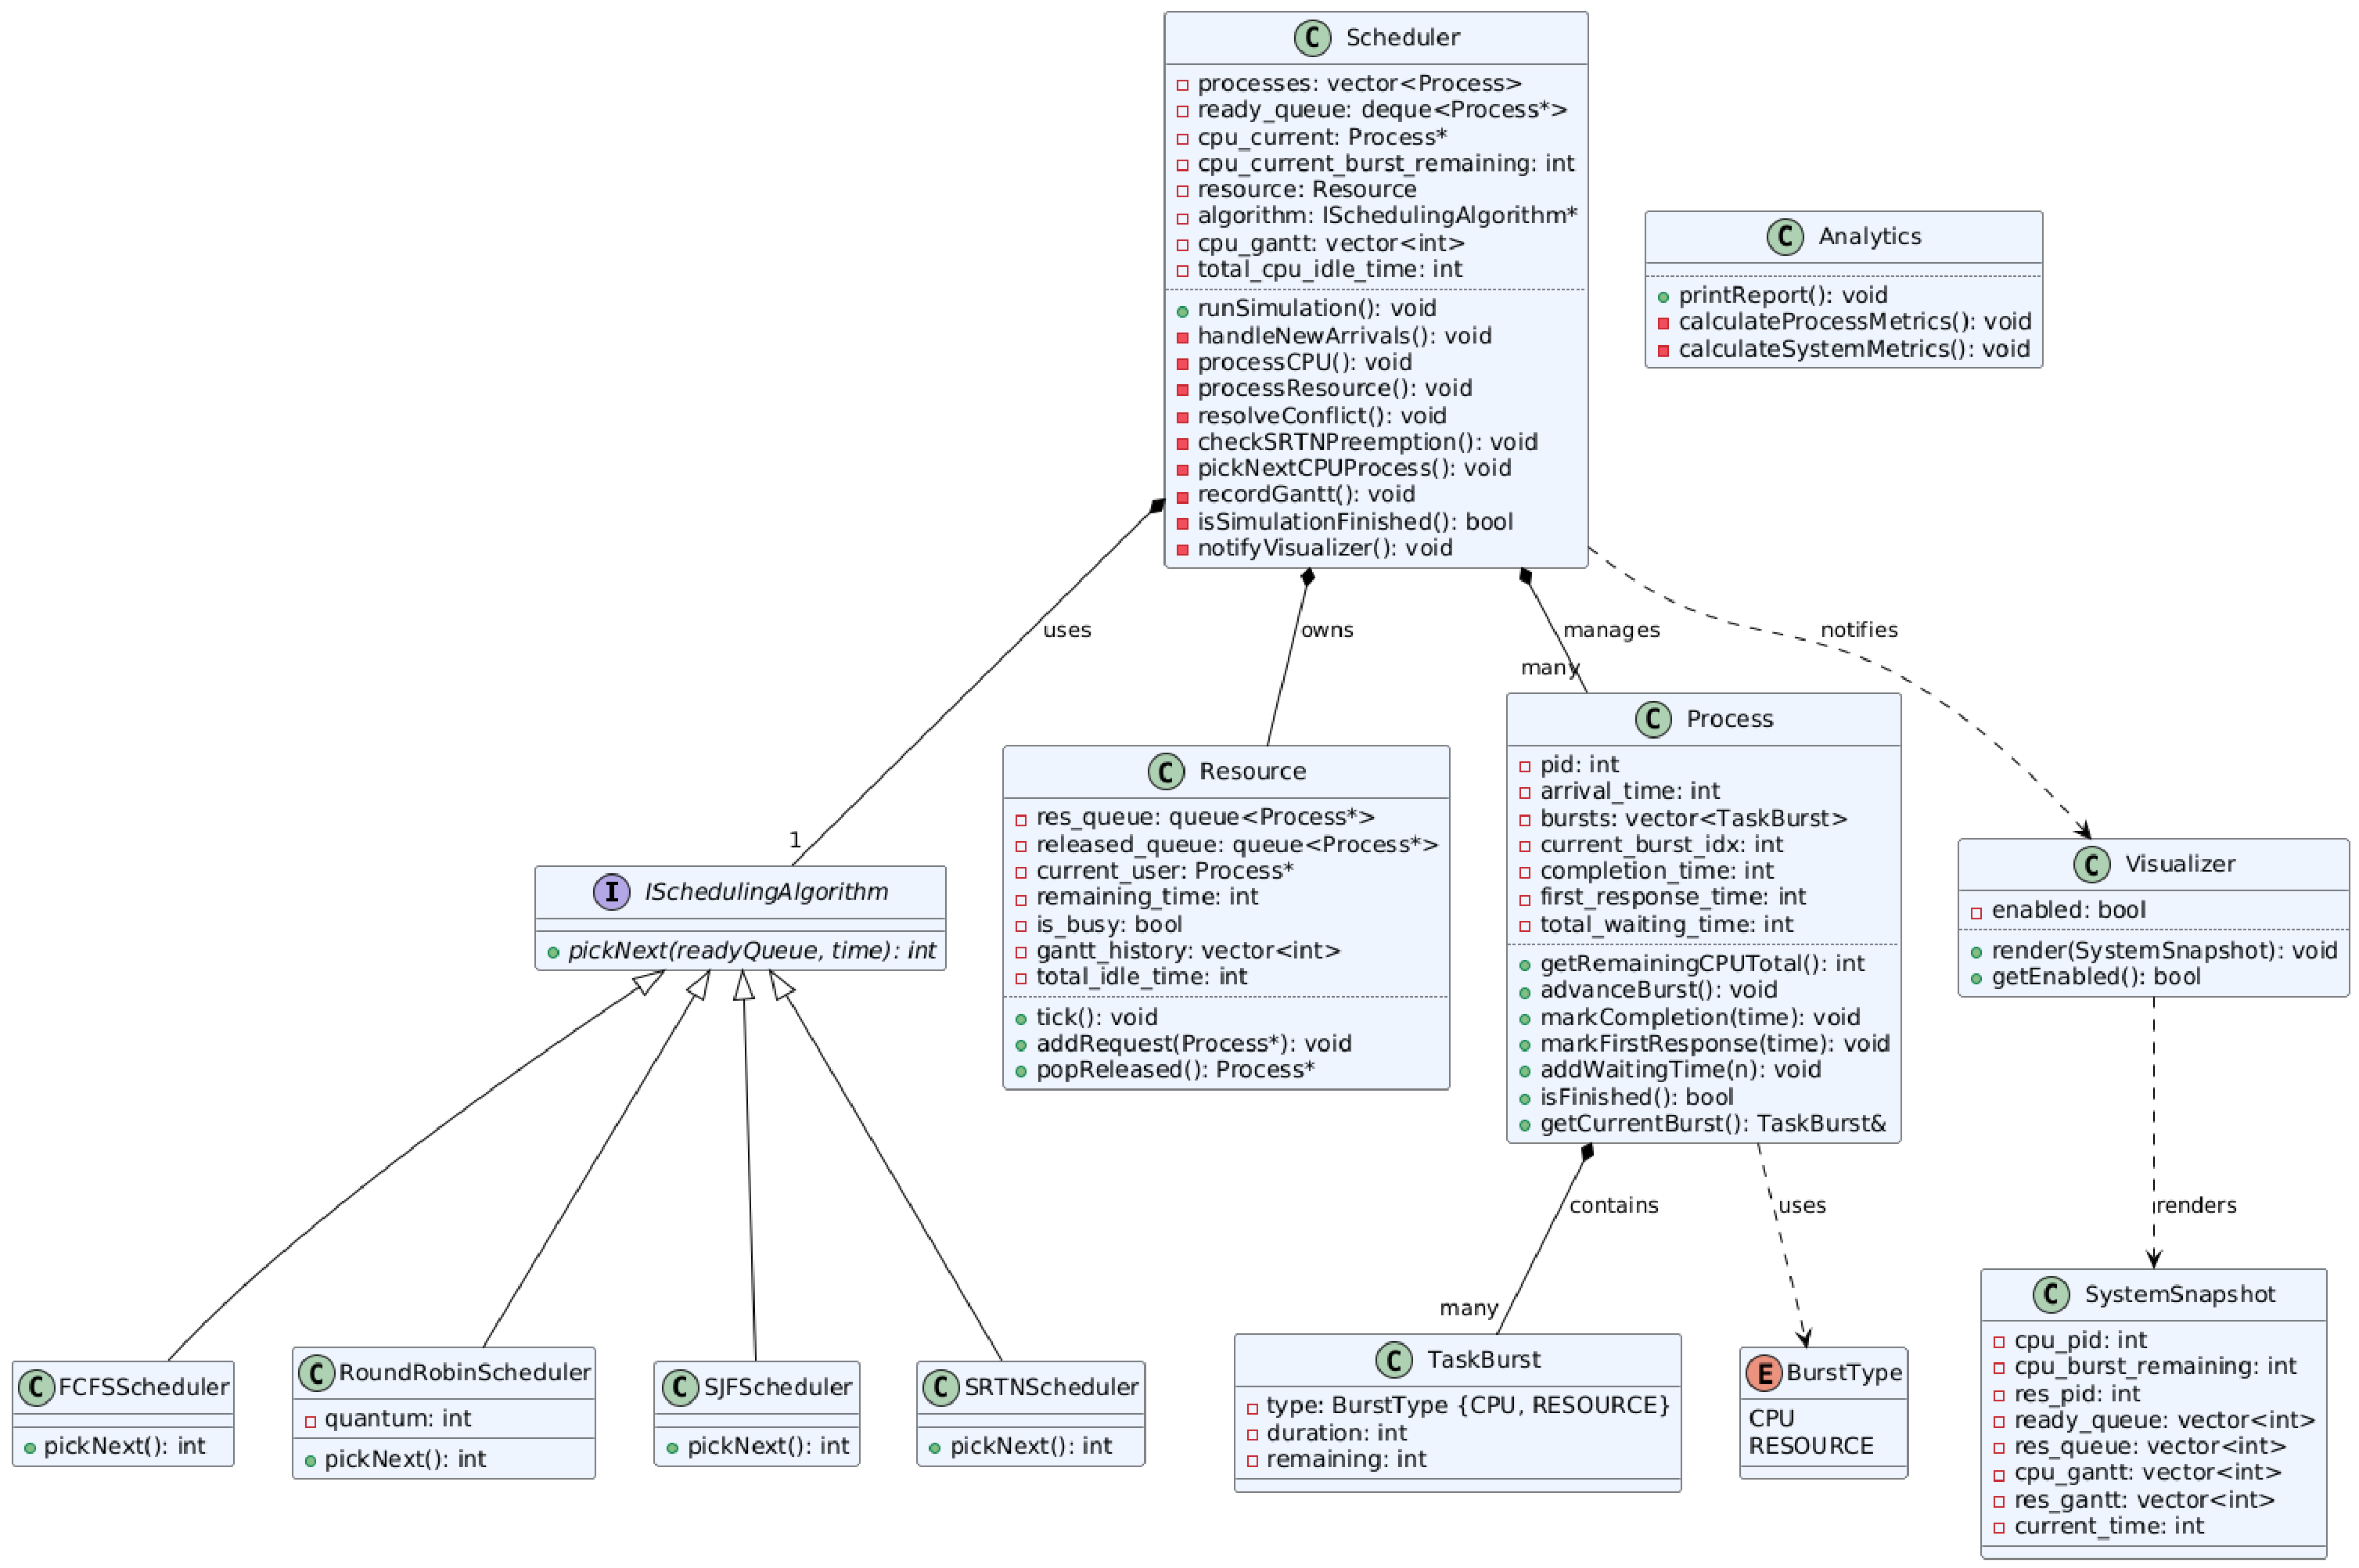
\includegraphics[width=\textwidth]{figures/class_diagram.pdf}
\caption{Class Diagram của chương trình}
\label{fig:class-diagram}
\end{figure}

\section{Sequence Diagram}

Hình~\ref{fig:sequence} mô tả luồng hoạt động chính của chương trình từ khi nhận tham số dòng lệnh đến khi xuất kết quả.

\begin{figure}[h]
\centering
\begin{tikzpicture}[node distance=0.5cm]
\tikzstyle{obj}=[rectangle, draw, minimum width=2cm, minimum height=0.7cm, rounded corners, font=\small]
\tikzstyle{line}=[thick]
\tikzstyle{arrow}=[->, thick]
\tikzstyle{return}=[<-, thick, dashed]

% Objects
\node[obj, fill=orange!20] (main) {main()};
\node[obj, right=3cm of main, fill=green!20] (parser) {:Parser};
\node[obj, right=3cm of parser, fill=blue!20] (scheduler) {:Scheduler};
\node[obj, right=3cm of scheduler, fill=red!20] (algo) {:Algorithm};

% Lifelines
\draw[line] (main.south) -- ++(0,-10cm);
\draw[line] (parser.south) -- ++(0,-10cm);
\draw[line] (scheduler.south) -- ++(0,-10cm);
\draw[line] (algo.south) -- ++(0,-10cm);

% Messages
\draw[arrow] ([yshift=-0.5cm]main.south) -- node[above, font=\tiny] {parseInput(path)} ([yshift=-0.5cm]parser.south);
\draw[return] ([yshift=-1cm]parser.south) -- node[above, font=\tiny] {vector<Process>} ([yshift=-1cm]main.south);

\draw[arrow] ([yshift=-1.8cm]main.south) -- node[above, font=\tiny] {new Scheduler(procs, algo)} ([yshift=-1.8cm]scheduler.south);

\draw[arrow] ([yshift=-2.8cm]main.south) -- node[above, font=\tiny] {runSimulation()} ([yshift=-2.8cm]scheduler.south);

% Loop box
\draw[thick, dashed] ([xshift=-2mm, yshift=-3.5cm]scheduler.south) rectangle ([xshift=2mm, yshift=-8cm]scheduler.south);
\node[font=\tiny] at ([yshift=-3.2cm]scheduler.south) {Loop per tick};

\draw[arrow] ([yshift=-4cm]scheduler.south) -- node[above, font=\tiny] {pickNext(queue)} ([yshift=-4cm]algo.south);
\draw[return] ([yshift=-4.5cm]algo.south) -- node[above, font=\tiny] {int idx} ([yshift=-4.5cm]scheduler.south);

\node[font=\tiny] at ([yshift=-6.5cm]scheduler.south) {Process CPU / Resource};

\draw[arrow] ([yshift=-9cm]main.south) -- node[above, font=\tiny] {writeOutput()} ([yshift=-9cm]parser.south);

\end{tikzpicture}
\caption{Sequence Diagram luồng chính}
\label{fig:sequence}
\end{figure}

\section{Cấu trúc dữ liệu}

\subsection{Hàng đợi Ready (Ready Queue)}

Hàng đợi ready được cài đặt bằng \code{std::deque<Process*>} (double-ended queue). Hàng đợi này hỗ trợ thêm phần tử ở cuối (khi tiến trình vào ready) và lấy phần tử ở đầu (khi CPU pick next process). Khi có xung đột (nhiều tiến trình vào ready cùng lúc), tiến trình mới đến được ưu tiên trước tiến trình trả về từ Resource R.

\subsection{Hàng đợi Resource}

Tài nguyên R duy trì hai hàng đợi \code{std::queue<Process*>}:
\begin{itemize}
    \item \textbf{res\_queue:} Hàng đợi FCFS các tiến trình đang chờ tài nguyên R.
    \item \textbf{released\_queue:} Hàng đợi các tiến trình vừa hoàn thành Resource burst, chờ được đưa trở lại ready queue.
\end{itemize}

\subsection{Hệ thống Snapshot cho TUI}

Cấu trúc \code{SystemSnapshot} được truyền từ \code{Scheduler} đến \code{Visualizer} mỗi tick, chứa toàn bộ trạng thái hiện tại:
\begin{itemize}
    \item Tiến trình đang chạy trên CPU (PID + burst còn lại).
    \item Tiến trình đang sử dụng Resource R.
    \item Danh sách các tiến trình trong ready queue.
    \item Danh sách các tiến trình trong resource queue.
    \item Lịch sử Gantt đã ghi nhận.
\end{itemize}

\chapter{Giải thích cài đặt}

\section{Entry point -- \texttt{main.cpp}}

File \code{src/main.cpp} là điểm vào của chương trình. Nó xử lý tham số dòng lệnh (hoặc hiển thị menu tương tác), khởi tạo các đối tượng và điều phối luồng chạy.

\begin{lstlisting}
int main(int argc, char* argv[]) {
    // Xu ly tham so dong lenh hoac menu
    if (argc > 1) {
        // CLI mode: <input> <output> <algo> [quantum] [--tui]
    } else {
        // Interactive menu mode
    }
    
    // Doc input
    auto processes = Parser::parseInput(input_path);
    
    // Tao thuat toan (unique_ptr)
    std::unique_ptr<ISchedulingAlgorithm> algo;
    switch (algo_code) {
        case 1: algo = std::make_unique<FCFSScheduler>(); break;
        case 2: algo = std::make_unique<RoundRobinScheduler>(quantum); break;
        case 3: algo = std::make_unique<SJFScheduler>(); break;
        case 4: algo = std::make_unique<SRTNScheduler>(); break;
    }
    
    // Khoi tao Scheduler va chay mo phong
    Scheduler scheduler(processes, algo.get());
    scheduler.runSimulation();
    
    // Ghi output va in analytics
    Parser::writeOutput(cpu_gantt, res_gantt, output_path);
    Analytics analytics(...);
    analytics.printReport();
}
\end{lstlisting}

Điểm đáng chú ý là việc sử dụng \code{std::unique\_ptr} thay vì \code{new}/\code{delete} để quản lý bộ nhớ cho đối tượng thuật toán. Điều này đảm bảo không rò rỉ bộ nhớ ngay cả khi ngoại lệ xảy ra (bug BUG-8 đã được sửa).

\section{Vòng lặp mô phỏng chính -- \texttt{runSimulation()}}

Đây là trái tim của chương trình. Mỗi tick (một đơn vị thời gian), vòng lặp thực hiện 10 bước theo thứ tự nghiêm ngặt.

\begin{figure}[h]
\centering
\begin{tikzpicture}[node distance=0.7cm, scale=0.75, transform shape]
\tikzstyle{startstop}=[ellipse, draw, fill=red!20, minimum width=1.8cm, minimum height=0.8cm, align=center]
\tikzstyle{process}=[rectangle, draw, fill=blue!15, minimum width=5cm, minimum height=0.8cm, rounded corners, align=center]
\tikzstyle{decision}=[diamond, draw, fill=yellow!20, minimum width=2cm, minimum height=1.2cm, aspect=2, align=center, text width=2cm]
\tikzstyle{arrow}=[->, thick]

\node[startstop] (start) {Start};
\node[decision, below=1.2cm of start] (finished) {isSimulation\\ Finished?};
\node[process, below=1.5cm of finished] (arrivals) {handleNewArrivals()};
\node[process, below=0.5cm of arrivals] (resource) {processResource()};
\node[process, below=0.5cm of resource] (conflict) {resolveConflict()};
\node[decision, right=4cm of finished] (srtn) {Algorithm\\ == SRTN?};
\node[process, below=1.5cm of srtn] (checkPreempt) {checkSRTN\\ Preemption()};
\node[process, below=0.5cm of checkPreempt] (pickNext) {pickNextCPU\\ Process()};
\node[process, below=0.5cm of pickNext] (gantt) {recordGantt()};
\node[process, below=0.5cm of gantt] (cpu) {processCPU()};
\node[process, below=0.5cm of cpu] (visual) {notifyVisualizer()};
\node[process, below=0.5cm of visual] (wait) {addWaitingTime()};
\node[process, below=0.5cm of wait] (tick) {++current\_time};
\node[startstop, below=0.8cm of tick] (end) {End};

\draw[arrow] (start) -- (finished);
\draw[arrow] (finished.west) -- ++(-1.5,0) node[above, font=\tiny] {No} |- (arrivals.west);
\draw[arrow] (arrivals) -- (resource);
\draw[arrow] (resource) -- (conflict);
\draw[arrow] (conflict) -| (srtn);
\draw[arrow] (srtn.south) -- node[right, font=\tiny] {Yes} (checkPreempt);
\draw[arrow] (checkPreempt) -- (pickNext);
\draw[arrow] (srtn.west) -- ++(-1,0) node[above, font=\tiny] {No} |- (pickNext);
\draw[arrow] (pickNext) -- (gantt);
\draw[arrow] (gantt) -- (cpu);
\draw[arrow] (cpu) -- (visual);
\draw[arrow] (visual) -- (wait);
\draw[arrow] (wait) -- (tick);
\draw[arrow] (tick) -- (finished.west-|tick.west) -- (finished.west);
\draw[arrow] (finished) -- node[right, font=\tiny] {Yes} ++(0,-1.2) -| (end);

\end{tikzpicture}
\caption{Flowchart vòng lặp mô phỏng chính}
\label{fig:sim-loop}
\end{figure}

\subsection{Chi tiết từng bước}

\begin{enumerate}
    \item \textbf{isSimulationFinished():} Kiểm tra điều kiện dừng -- CPU idle, ready queue rỗng, resource idle, resource queue rỗng, và tất cả tiến trình đã kết thúc.
    
    \item \textbf{handleNewArrivals():} Duyệt danh sách tiến trình, đưa các tiến trình có\\ \phantom{\textbf{handleNewArrivals():}} \code{arrival\_time == current\_time} vào hàng đợi arrivals tạm thời.
    
    \item \textbf{processResource():} Gọi \code{Resource::tick()} -- ghi nhận trạng thái resource vào Gantt, decrement burst nếu đang chạy, xử lý hoàn thành, và khởi động tiến trình mới từ hàng đợi nếu resource rảnh. Sau đó đưa các tiến trình vừa hoàn thành Resource burst vào hàng đợi return.
    
    \item \textbf{resolveConflict():} Đưa tiến trình arrivals vào ready queue trước, sau đó đến tiến trình từ resource return. \textbf{Tiến trình mới đến được ưu tiên trước.}
    
    \item \textbf{checkSRTNPreemption():} Chỉ áp dụng với SRTN. Nếu có tiến trình trong ready queue có tổng CPU còn lại nhỏ hơn tiến trình đang chạy, tiến trình đang chạy bị preempt.
    
    \item \textbf{pickNextCPUProcess():} Nếu CPU rảnh và ready queue không rỗng, gọi\\ \phantom{\textbf{pickNextCPUProcess():}} \code{algorithm->pickNext()} để chọn tiến trình tiếp theo.
    
    \item \textbf{recordGantt():} Ghi PID của tiến trình đang chạy (hoặc -1 nếu idle) vào \code{cpu\_gantt}.
    
    \item \textbf{processCPU():} Decrement burst của tiến trình đang chạy. Xử lý hoàn thành burst (chuyển sang R hoặc kết thúc), hoặc preemption do hết quantum RR.
    
    \item \textbf{notifyVisualizer():} Nếu bật TUI, gửi snapshot trạng thái đến Visualizer.
    
    \item \textbf{addWaitingTime():} Mỗi tiến trình trong ready queue được tăng waiting time thêm 1.
\end{enumerate}

\section{Cơ chế hoạt động của Resource}

\begin{lstlisting}[caption={Resource::tick() -- xu\^at Gantt truoc decrement}]
void Resource::tick() {
    // Buoc 1: Ghi nhan trang thai vao Gantt (dau tick)
    gantt_history.push_back(current_user ? current_user->id : -1);
    if (!is_busy) ++total_idle_time;
    
    // Buoc 2: Decrement neu dang chay
    if (is_busy) {
        --remaining_time;
        --current_user->getCurrentBurst().remaining;
    }
    
    // Buoc 3: Ket thuc burst
    if (is_busy && remaining_time <= 0) {
        current_user->advanceBurst();
        released_queue.push(current_user);
        current_user = nullptr;
        is_busy = false;
    }
    
    // Buoc 4: Khoi dong tien trinh moi tu hang doi
    if (!is_busy && !res_queue.empty()) {
        current_user = res_queue.front();
        res_queue.pop();
        remaining_time = current_user->getCurrentBurst().remaining;
        is_busy = true;
    }
}
\end{lstlisting}

Thứ tự các bước trong \code{tick()} rất quan trọng. Gantt được ghi ở \textbf{đầu tick} (trước decrement) để phản ánh đúng trạng thái của tick đó. Đây là kết quả sửa lỗi BUG-R1.

\subsection{Xử lý hoàn thành Resource burst}

Khi một tiến trình hoàn thành Resource burst, nó được đưa vào \code{released\_queue}. Scheduler sau đó sẽ đưa tiến trình này trở lại ready queue:
\begin{itemize}
    \item Nếu tiến trình đã hoàn thành tất cả các burst (CPU và R): gọi \linebreak[4]\code{markCompletion(current\_time + 1)}.
    \item Nếu còn burst: đưa vào ready queue thông qua \code{r\_returnees\_this\_tick}.
\end{itemize}

\section{Cơ chế Preemption}

\subsection{Preemption trong Round Robin}

Preemption RR được xử lý trong \code{processCPU()}:

\begin{lstlisting}
void Scheduler::processCPU() {
    if (!cpu_current) return;
    
    --cpu_current_burst_remaining;
    --cpu_current->getCurrentBurst().remaining;
    
    if (cpu_algorithm == ROUND_ROBIN) --cpu_rr_quantum_counter;
    
    // 1. Hoan thanh burst
    if (cpu_current_burst_remaining <= 0) {
        cpu_current->advanceBurst();
        if (cpu_current->isFinished()) {
            cpu_current->markCompletion(current_time + 1);
        } else {
            resource.addRequest(cpu_current);
        }
        cpu_current = nullptr;
        cpu_rr_quantum_counter = 0;
        return;
    }
    
    // 2. RR preemption
    if (cpu_algorithm == ROUND_ROBIN && cpu_rr_quantum_counter <= 0) {
        ready_queue.push_back(cpu_current);
        cpu_current = nullptr;
        cpu_rr_quantum_counter = quantum;
        return;
    }
}
\end{lstlisting}

Khi quantum RR hết (đếm ngược về 0) và CPU burst chưa kết thúc, tiến trình bị đẩy trở lại cuối ready queue.

\subsection{Preemption trong SRTN}

\begin{lstlisting}
void Scheduler::checkSRTNPreemption() {
    if (cpu_algorithm != SRTN) return;
    if (!cpu_current || ready_queue.empty()) return;
    
    int current_rem = cpu_current->getRemainingCPUTotal();
    
    for (size_t i = 0; i < ready_queue.size(); ++i) {
        int rem = ready_queue[i]->getRemainingCPUTotal();
        if (rem < current_rem) {
            // Preempt!
            ready_queue.push_back(cpu_current);
            cpu_current = nullptr;
            return;
        }
    }
}
\end{lstlisting}

Việc so sánh sử dụng \code{getRemainingCPUTotal()} (tổng thời gian CPU còn lại của tất cả các CPU burst trong tương lai) thay vì chỉ burst hiện tại. Đây là kết quả sửa lỗi BUG-2.

\section{Các bug đã phát hiện và sửa}

Trong quá trình phát triển, 7 bug đã được phát hiện và sửa:

\begingroup
\renewcommand{\code}[1]{\texttt{\hyphenchar\font=45\relax#1}}
\begin{longtable}{|p{2cm}|>{\raggedright}p{4cm}|>{\raggedright\hyphenchar\font=45}p{4cm}|}
\hline
\textbf{Bug} & \textbf{Mô tả} & \textbf{Cách sửa} \\
\hline
\endhead
BUG-1 & CPU off-by-one: \code{processCPU()} chạy trước \code{recordGantt()} & Đổi thứ tự loop, \linebreak[4]\code{markCompletion(current\_time + 1)} \\
\hline
BUG-2 & SRTN so sánh \code{currentBurst.remaining} thay vì \linebreak[4]\code{getRemainingCPUTotal()} & Dùng \code{getRemainingCPUTotal()} cho cả 2 vế \\
\hline
BUG-3 & \code{markCompletion} không đồng nhất giữa CPU và Resource path & Cả 2 đều dùng \code{current\_time + 1} \\
\hline
BUG-4 & RR quantum bị +1 tick & Tự động sửa cùng BUG-1 \\
\hline
BUG-5 & Idle tick thừa ở cuối simulation & Chuyển \linebreak[4]\code{isSimulationFinished()} lên đầu loop \\
\hline
BUG-8 & Memory leak khi exception & Dùng \code{unique\_ptr} thay \code{new}/\code{delete} \\
\hline
BUG-R1 & Resource off-by-one: ghi Gantt sai thứ tự & Ghi Gantt trước decrement \\
\hline
\end{longtable}
\endgroup

\chapter{Kết quả thực nghiệm}

\section{Môi trường thử nghiệm}

\begin{itemize}
    \item \textbf{Hệ điều hành:} Ubuntu 24.04 (Noble Numbat)
    \item \textbf{Trình biên dịch:} g++ (GCC) 13.2.0
    \item \textbf{Tiêu chuẩn C++:} C++17
    \item \textbf{CPU:} x86\_64
\end{itemize}

\section{Kết quả các test case}

Chương trình được kiểm tra với 7 bộ dữ liệu đầu vào. Dưới đây là kết quả biểu đồ Gantt cho từng bộ.

\subsection{Test case 1: \texttt{input\_basic.txt} (FCFS)}

Đầu vào: 3 tiến trình với chu kỳ CPU-R đan xen.

\begin{itemize}
    \item P1: đến 0, bursts [CPU 5, R 3, CPU 2, R 2]
    \item P2: đến 2, bursts [CPU 4, R 2]
    \item P3: đến 5, bursts [CPU 3, R 1, CPU 2, R 1]
\end{itemize}

\begin{verbatim}
CPU: 1 1 1 1 1 2 2 2 2 3 3 3 1 1 3 3 _ _
R  : _ _ _ _ _ _ 1 1 1 _ 2 2 _ 3 _ 1 1 3
\end{verbatim}

Tổng thời gian mô phỏng: 18 ticks. CPU utilization: 88,88\%. Resource utilization: 50,00\%.

\begin{table}[h]
\centering
\begin{tabular}{|c|c|c|c|}
\hline
PID & Response (s) & Waiting (s) & Turnaround (s) \\
\hline
P1 & 0,00 & 4,00 & 17,00 \\
P2 & 3,00 & 3,00 & 10,00 \\
P3 & 4,00 & 5,00 & 13,00 \\
\hline
TB & 2,33 & 4,00 & 13,33 \\
\hline
\end{tabular}
\caption{Kết quả test case 1}
\end{table}

\subsection{Test case 2: \texttt{input\_simple.txt} (FCFS)}

Đầu vào: 2 tiến trình CPU-only.

\begin{itemize}
    \item P1: đến 0, bursts [CPU 3]
    \item P2: đến 1, bursts [CPU 5]
\end{itemize}

\begin{verbatim}
CPU: 1 1 1 2 2 2 2 2
R  : _ _ _ _ _ _ _ _
\end{verbatim}

CPU utilization: 100\%. Resource utilization: 0\%.

\begin{table}[h]
\centering
\begin{tabular}{|c|c|c|c|}
\hline
PID & Response (s) & Waiting (s) & Turnaround (s) \\
\hline
P1 & 0,00 & 0,00 & 3,00 \\
P2 & 2,00 & 2,00 & 7,00 \\
\hline
TB & 1,00 & 1,00 & 5,00 \\
\hline
\end{tabular}
\caption{Kết quả test case 2}
\end{table}

\subsection{Test case 3: \texttt{input\_fcfs.txt} (FCFS)}

Đầu vào: 3 tiến trình với resource R.

\begin{itemize}
    \item P1: đến 0, bursts [CPU 5, R 2]
    \item P2: đến 2, bursts [CPU 3]
    \item P3: đến 4, bursts [CPU 4, R 3]
\end{itemize}

\begin{verbatim}
CPU: 1 1 1 1 1 2 2 2 3 3 3 3 _ _ _ _
R  : _ _ _ _ _ _ 1 1 _ _ _ _ _ 3 3 3
\end{verbatim}

CPU utilization: 75\%. Resource utilization: 31,25\%.

\begin{table}[h]
\centering
\begin{tabular}{|c|c|c|c|}
\hline
PID & Response (s) & Waiting (s) & Turnaround (s) \\
\hline
P1 & 0,00 & 0,00 & 8,00 \\
P2 & 3,00 & 3,00 & 6,00 \\
P3 & 4,00 & 4,00 & 12,00 \\
\hline
TB & 2,33 & 2,33 & 8,67 \\
\hline
\end{tabular}
\caption{Kết quả test case 3}
\end{table}

\subsection{Test case 4: \texttt{input\_rr.txt} (RR, quantum = 2)}

Đầu vào: 3 tiến trình CPU-only đến cùng lúc.

\begin{itemize}
    \item P1: đến 0, bursts [CPU 6]
    \item P2: đến 0, bursts [CPU 3]
    \item P3: đến 0, bursts [CPU 4]
\end{itemize}

\begin{verbatim}
CPU: 1 1 2 2 3 3 1 1 2 3 3 1 1
R  : _ _ _ _ _ _ _ _ _ _ _ _ _
\end{verbatim}

CPU utilization: 100\%. Resource utilization: 0\%.

\begin{table}[h]
\centering
\begin{tabular}{|c|c|c|c|}
\hline
PID & Response (s) & Waiting (s) & Turnaround (s) \\
\hline
P1 & 0,00 & 9,00 & 13,00 \\
P2 & 2,00 & 7,00 & 9,00 \\
P3 & 4,00 & 8,00 & 11,00 \\
\hline
TB & 2,00 & 8,00 & 11,00 \\
\hline
\end{tabular}
\caption{Kết quả test case 4}
\end{table}

\subsection{Test case 5: \texttt{input\_sjf.txt} (SJF)}

Đầu vào: 4 tiến trình CPU-only đến so le.

\begin{itemize}
    \item P1: đến 0, bursts [CPU 8]
    \item P2: đến 1, bursts [CPU 4]
    \item P3: đến 2, bursts [CPU 2]
    \item P4: đến 3, bursts [CPU 1]
\end{itemize}

\begin{verbatim}
CPU: 1 1 1 1 1 1 1 1 4 3 3 2 2 2 2
R  : _ _ _ _ _ _ _ _ _ _ _ _ _ _ _
\end{verbatim}

CPU utilization: 100\%. Resource utilization: 0\%.

\begin{table}[h]
\centering
\begin{tabular}{|c|c|c|c|}
\hline
PID & Response (s) & Waiting (s) & Turnaround (s) \\
\hline
P1 & 0,00 & 0,00 & 8,00 \\
P2 & 10,00 & 10,00 & 14,00 \\
P3 & 7,00 & 7,00 & 9,00 \\
P4 & 5,00 & 5,00 & 6,00 \\
\hline
TB & 5,50 & 5,50 & 9,25 \\
\hline
\end{tabular}
\caption{Kết quả test case 5}
\end{table}

\subsection{Test case 6: \texttt{input\_srtn.txt} (SRTN)}

Đầu vào: 3 tiến trình CPU-only đến so le.

\begin{itemize}
    \item P1: đến 0, bursts [CPU 8]
    \item P2: đến 1, bursts [CPU 3]
    \item P3: đến 2, bursts [CPU 2]
\end{itemize}

\begin{verbatim}
CPU: 1 2 2 2 3 3 1 1 1 1 1 1 1
R  : _ _ _ _ _ _ _ _ _ _ _ _ _
\end{verbatim}

CPU utilization: 100\%. Resource utilization: 0\%.

\begin{table}[h]
\centering
\begin{tabular}{|c|c|c|c|}
\hline
PID & Response (s) & Waiting (s) & Turnaround (s) \\
\hline
P1 & 0,00 & 5,00 & 13,00 \\
P2 & 0,00 & 0,00 & 3,00 \\
P3 & 2,00 & 2,00 & 4,00 \\
\hline
TB & 0,67 & 2,33 & 6,67 \\
\hline
\end{tabular}
\caption{Kết quả test case 6}
\end{table}

\subsection{Test case 7: \texttt{input\_bug2\_srtn.txt} (SRTN)}

Đầu vào: 2 tiến trình, P1 có chu kỳ CPU-R-CPU.

\begin{itemize}
    \item P1: đến 0, bursts [CPU 2, R 1, CPU 8]
    \item P2: đến 1, bursts [CPU 5]
\end{itemize}

\begin{verbatim}
CPU: 1 2 2 2 2 2 1 _ 1 1 1 1 1 1 1 1
R  : _ _ _ _ _ _ _ _ 1 _ _ _ _ _ _ _
\end{verbatim}

CPU utilization: 93,75\%. Resource utilization: 6,25\%.

\begin{table}[h]
\centering
\begin{tabular}{|c|c|c|c|}
\hline
PID & Response (s) & Waiting (s) & Turnaround (s) \\
\hline
P1 & 0,00 & 5,00 & 16,00 \\
P2 & 0,00 & 0,00 & 5,00 \\
\hline
TB & 0,00 & 2,50 & 10,50 \\
\hline
\end{tabular}
\caption{Kết quả test case 7}
\end{table}

\section{So sánh các thuật toán}

Để so sánh các thuật toán, chúng tôi sử dụng test case 4 (input\_rr.txt) -- 3 tiến trình đến cùng lúc -- và test case 6 (input\_srtn.txt) -- 3 tiến trình đến so le -- vì đây là các kịch bản thể hiện rõ sự khác biệt giữa các thuật toán.

\subsection{So sánh trên test case 4 (cùng đến)}

\begin{table}[h]
\centering
\begin{tabular}{|c|c|c|c|c|}
\hline
Thuật toán & RT TB & WT TB & TAT TB & CPU Util \\
\hline
FCFS & 0,00 & 5,00 & 9,67 & 100\% \\
RR (q=2) & 2,00 & 8,00 & 11,00 & 100\% \\
SJF & 0,00 & 5,00 & 9,67 & 100\% \\
SRTN & 0,00 & 5,00 & 9,67 & 100\% \\
\hline
\end{tabular}
\caption{So sánh các thuật toán trên test case 4}
\end{table}

Khi tất cả tiến trình đến cùng lúc, SJF và SRTN cho kết quả tương đương FCFS (đều chạy P1 trước). RR có waiting time và turnaround time cao hơn do overhead của preemption và context-switch.

\subsection{So sánh trên test case 6 (đến so le)}

\begin{table}[h]
\centering
\begin{tabular}{|c|c|c|c|c|}
\hline
Thuật toán & RT TB & WT TB & TAT TB & CPU Util \\
\hline
FCFS & 1,33 & 4,67 & 9,00 & 100\% \\
RR (q=2) & 1,33 & 5,00 & 9,33 & 100\% \\
SJF & 0,67 & 2,33 & 6,67 & 100\% \\
SRTN & 0,67 & 2,33 & 6,67 & 100\% \\
\hline
\end{tabular}
\caption{So sánh các thuật toán trên test case 6}
\end{table}

Khi tiến trình đến so le với burst length khác nhau, SJF và SRTN cho thấy ưu thế vượt trội: waiting time giảm gần một nửa so với FCFS và RR.

\begin{figure}[h]
\centering
\begin{tikzpicture}[scale=0.8]
\definecolor{bar1}{RGB}{66,133,244}
\definecolor{bar2}{RGB}{219,68,55}
\definecolor{bar3}{RGB}{244,180,0}
\definecolor{bar4}{RGB}{15,157,88}

% Axes
\draw[thick,->] (0,0) -- (10,0);
\draw[thick,->] (0,0) -- (0,5.5);

% Labels
\node[left] at (0,0) {0};
\node[left] at (0,1) {2};
\node[left] at (0,2) {4};
\node[left] at (0,3) {6};
\node[left] at (0,4) {8};
\node[left] at (0,5) {10};

% FCFS
\draw[fill=bar1] (0.5,0) rectangle (2.5,{4.67/2});
\node[rotate=90] at (1.5,{4.67/4+0.3}) {FCFS};
\node at (1.5,{4.67/2+0.4}) {4,67};

% RR
\draw[fill=bar2] (3,0) rectangle (5,{5.0/2});
\node[rotate=90] at (4,{5.0/4+0.3}) {RR};
\node at (4,{5.0/2+0.4}) {5,00};

% SJF
\draw[fill=bar3] (5.5,0) rectangle (7.5,{2.33/2});
\node[rotate=90] at (6.5,{2.33/4+0.3}) {SJF};
\node at (6.5,{2.33/2+0.4}) {2,33};

% SRTN
\draw[fill=bar4] (8,0) rectangle (10,{2.33/2});
\node[rotate=90] at (9,{2.33/4+0.3}) {SRTN};
\node at (9,{2.33/2+0.4}) {2,33};

\draw[thick] (0,{4.67/2}) -- (10,{4.67/2}) node[right] {FCFS/RR};

\end{tikzpicture}
\caption{So sánh Waiting Time trung bình giữa các thuật toán (test case 6)}
\label{fig:wt-comparison}
\end{figure}

\subsection{Nhận xét}

\begin{enumerate}
    \item \textbf{SJF và SRTN} cho kết quả vượt trội về waiting time và turnaround time so với FCFS và RR, đặc biệt khi các tiến trình có burst length chênh lệch lớn.
    \item \textbf{Round Robin} có waiting time cao nhất do cơ chế preemption định kỳ, nhưng đảm bảo tính công bằng -- không tiến trình nào bị starvation.
    \item \textbf{FCFS} đơn giản nhưng dễ bị hiệu ứng convoy: tiến trình CPU burst dài ở đầu hàng đợi sẽ làm tăng waiting time của các tiến trình khác.
    \item \textbf{CPU Utilization} đạt 100\% trong hầu hết test case CPU-only. Với các test case có resource R, utilization thấp hơn do CPU phải chờ resource.
\end{enumerate}

\chapter{Kết luận}

\section{Kết quả đạt được}

Đồ án đã hoàn thành các mục tiêu đề ra:

\begin{enumerate}
    \item \textbf{Xây dựng thành công chương trình mô phỏng} điều phối tiến trình với 4 thuật toán FCFS, Round Robin, SJF và SRTN.
    \item \textbf{Hỗ trợ tài nguyên dùng chung R} với cơ chế FCFS, cho phép mô phỏng các kịch bản CPU-R đan xen.
    \item \textbf{Xuất biểu đồ Gantt} cho cả CPU và tài nguyên R, giúp trực quan hóa quá trình điều phối.
    \item \textbf{Phân tích hiệu năng} với đầy đủ các chỉ số response time, waiting time, turnaround time và utilization.
    \item \textbf{Giao diện TUI} real-time cho phép quan sát quá trình mô phỏng theo từng tick.
    \item \textbf{Phát hiện và sửa 7 bug}, đảm bảo tính chính xác của chương trình.
\end{enumerate}

\section{Hạn chế}

Bên cạnh những kết quả đạt được, đồ án còn một số hạn chế:

\begin{itemize}
    \item Chỉ hỗ trợ một tài nguyên R duy nhất, chưa mở rộng được cho nhiều tài nguyên.
    \item Chưa triển khai các thuật toán điều phối nâng cao như MLFQ hay Priority Scheduling.
    \item Chưa tính đến context-switch overhead -- trong thực tế, mỗi lần chuyển đổi tiến trình tốn một khoảng thời gian nhất định.
    \item Chưa có cơ chế phát hiện starvation, đặc biệt quan trọng với SJF và SRTN.
    \item Các thành viên dữ liệu trong hầu hết các lớp đều là public, chưa tuân thủ nghiêm ngặt tính đóng gói.
\end{itemize}

\section{Hướng phát triển}

Trong tương lai, chương trình có thể được mở rộng theo các hướng sau:

\begin{itemize}
    \item \textbf{MLFQ (Multi-Level Feedback Queue):} Thuật toán điều phối được sử dụng trong nhiều hệ điều hành hiện đại (BSD, Solaris), cho phép tiến trình di chuyển giữa các queue có độ ưu tiên khác nhau dựa trên hành vi CPU-bound hay I/O-bound.
    \item \textbf{Priority Scheduling:} Thêm trường độ ưu tiên vào tiến trình, cho phép điều phối theo mức độ ưu tiên.
    \item \textbf{Chế độ batch:} Chạy tự động nhiều test case và xuất kết quả dạng CSV/JSON để so sánh.
    \item \textbf{Starvation detection:} Cảnh báo khi một tiến trình chờ quá lâu (vượt ngưỡng).
    \item \textbf{Context-switch overhead:} Thêm tham số thời gian chuyển đổi ngữ cảnh để mô phỏng thực tế hơn.
    \item \textbf{Cải thiện chất lượng mã nguồn:} Encapsulation, validation đầu vào, kiểm tra isatty cho ANSI codes, constants thay magic strings.
\end{itemize}

\begin{thebibliography}{99}

\bibitem{tanenbaum2015}
A.~S. Tanenbaum and H.~Bos,
\textit{Modern Operating Systems}, 4th~ed.
Pearson, 2015.

\bibitem{silberschatz2018}
A.~Silberschatz, P.~B. Galvin, and G.~Gagne,
\textit{Operating System Concepts}, 10th~ed.
Wiley, 2018.

\bibitem{stallings2018}
W.~Stallings,
\textit{Operating Systems: Internals and Design Principles}, 9th~ed.
Pearson, 2018.

\bibitem{cppreference}
cppreference.com,
\textit{C++ Standard Library Reference},
\url{https://en.cppreference.com/}

\end{thebibliography}

\chapter{Phụ lục}

\section{Hướng dẫn cài đặt và biên dịch}

\subsection{Yêu cầu hệ thống}

\begin{itemize}
    \item Trình biên dịch C++ hỗ trợ C++17 (g++ $\ge$ 8, clang $\ge$ 7)
    \item Make
\end{itemize}

\subsection{Biên dịch chương trình}

\begin{verbatim}
# Clone repository
git clone https://github.com/NguyenPhan161206/Process_Schedule_Algorithm.git
cd Process_Schedule_Algorithm

# Build
make

# Clean
make clean
\end{verbatim}

\subsection{Chạy chương trình}

\begin{verbatim}
# CLI mode
./scheduler test_cases/input_basic.txt output/gantt.txt 1

# Round Robin voi quantum 3
./scheduler test_cases/input_rr.txt output/gantt_rr.txt 2 3

# SRTN voi TUI
./scheduler test_cases/input_srtn.txt output/gantt_srtn.txt 4 --tui

# Interactive menu
./scheduler
\end{verbatim}

\subsection{Biên dịch báo cáo LaTeX}

\begin{verbatim}
cd report
xelatex main.tex
xelatex main.tex  % Chay 2 lan de cap nhat cross-reference
\end{verbatim}

\section{Mã nguồn các test case}

\subsection{\texttt{test\_cases/input\_basic.txt}}

\begin{verbatim}
3
0 5 3 2 2
2 4 2
5 3 1 2 1
\end{verbatim}

\subsection{\texttt{test\_cases/input\_simple.txt}}

\begin{verbatim}
2
0 3
1 5
\end{verbatim}

\subsection{\texttt{test\_cases/input\_fcfs.txt}}

\begin{verbatim}
3
0 5 2
2 3
4 4 3
\end{verbatim}

\subsection{\texttt{test\_cases/input\_rr.txt}}

\begin{verbatim}
3
0 6
0 3
0 4
\end{verbatim}

\subsection{\texttt{test\_cases/input\_sjf.txt}}

\begin{verbatim}
4
0 8
1 4
2 2
3 1
\end{verbatim}

\subsection{\texttt{test\_cases/input\_srtn.txt}}

\begin{verbatim}
3
0 8
1 3
2 2
\end{verbatim}

\subsection{\texttt{test\_cases/input\_bug2\_srtn.txt}}

\begin{verbatim}
2
0 2 1 8
1 5
\end{verbatim}


\end{document}
